\section{Свойства на изчислими реални функции}
Днес, 2024-05-08.
$\theta: \subseteq \R^N \to \R$ изчислима

Припомняме, че $\theta$ е изчислима, ако
\begin{equation}
    \begin{split}
        \forall \overrightarrow\xi \in \dom\theta,\ \forall f_1, \dots f_N,\ g_1, \dots, g_N,\ h_1, \dots, h_N: \N \to \N,\ \forall k,\ i:\; \left[\left| \frac{f_k(i) - g_k(i)}{h_k(i) + 1}\right| < \frac{1}{i+1} \right]\\
        \Longrightarrow \exists \underbrace{F, G, H}_{\text{изчислителна система}} \text{- изчислими оператори},\ \forall i:\; \\
        \left| \frac{F(\overrightarrow{f}, \overrightarrow{g}, \overrightarrow{h})(i) - G(\overrightarrow{f}, \overrightarrow{g}, \overrightarrow{h})(i)}{H(\overrightarrow{f}, \overrightarrow{g}, \overrightarrow{h})(i)} - \theta(\overrightarrow\xi)\right| < \frac{1}{i+1}
    \end{split}
\end{equation}
\subsection{Изчислителни системи на някои функции}
Сега ще намерим изчислителната система:
\begin{example}
    \begin{equation}
        \theta(\overrightarrow\xi) = \xi_k
    \end{equation}
    \begin{equation}
        \begin{split}
            F(f_1, g_1, h_1, \dots, f_N, g_N, h_n) = f_k \\
            G(f_1, g_1, h_1, \dots, f_N, g_N, h_n) = g_k \\
            H(f_1, g_1, h_1, \dots, f_N, g_N, h_n) = h_k
        \end{split}
    \end{equation}
\end{example}

\begin{example}
    \begin{equation}
        \theta(\xi) = -\xi
    \end{equation}
    И знаем, че:
    \begin{equation}
        \left|\frac{f(i) - g(i)}{h(i) + 1} - \xi\right| < \frac{1}{i+1}
    \end{equation}
    Тогава изчислителната система ще бъде:
    \begin{equation}
        \begin{split}
            F(f, g, h) = g \\
            G(f, g, h) = f \\
            H(f, g, h) = h
        \end{split}
    \end{equation}
    и имаме:
    \begin{equation}
        \left|\frac{g(i) - f(i)}{h(i) + 1} - (-\xi)\right| < \frac{1}{i+1}
    \end{equation}
\end{example}

\begin{example}
    \begin{equation}
        \theta(\xi) = |\xi|
    \end{equation}
    И знаем, че:
    \begin{equation}
        \left|\frac{f(i) - g(i)}{h(i) + 1} - \xi\right| < \frac{1}{i+1}
    \end{equation}
    Тогава изчислителната система ще бъде:
    \begin{equation}
        \begin{split}
            F(f, g, h) = |f - g| \\
            G(f, g, h) = 0 \\
            H(f, g, h) = h
        \end{split}
    \end{equation}
\end{example}
\begin{example}
    \begin{equation}
        \theta(\xi) = \alpha
    \end{equation}
    Където $\alpha \in \R$ - изчислимо:
    \begin{equation}
        \left|\frac{a(i) - b(i)}{c(i) + 1}- \alpha\right| < \frac{1}{i+1}
    \end{equation}
    Тогава изчислителната система ще бъде:
    \begin{equation}
        \begin{split}
            F(f, g, h) = a \\
            G(f, g, h) = b \\
            H(f, g, h) = c
        \end{split}
    \end{equation}
\end{example}

\subsection{Редици като реални функции}
\begin{proposition}
    Една редица $a: \N \to \R$ е изчислима $\iff$ $a: \subseteq \R \to \R$ е изчислима
\end{proposition}
\begin{proof}
    \begin{itemize}
        \item[$(\Rightarrow)$] $a: \N \to \R$ е изчислима, значи:
        \begin{equation}
            \exists u, v, w: \N^2 \to \N,\ \forall n, i \in \N:\; \left| \frac{u(n, i) - v(n, i)}{w(n, i) + 1} - a_n\right| < \frac{1}{i+1}
        \end{equation}
        Първи опит за изчислителна система
        \begin{equation}
            \begin{split}
                F(f, g, h) = u(n, i) \\
                G(f, g, h) = v(n, i) \\
                H(f, g, h) = w(n, i) \\
                n = ??
            \end{split}
        \end{equation}
        Можем да приближим $n$ по следния начин:
        \begin{equation}
            n = \left\lfloor \frac{f(1) - g(1)}{h(1) + 1} + \frac{1}{2}\right\rfloor = E(f, g, h)
        \end{equation}
        И ще заместим в горната система:
        \begin{equation}
            \begin{split}
                n = E(f,g,h) \\
                F(f, g, h) = u(n, i) \\
                G(f, g, h) = v(n, i) \\
                H(f, g, h) = w(n, i)
            \end{split}
        \end{equation}
        \item[$(\Leftarrow)$] Нека имаме изчислителна система $\langle F, G, H\rangle$ за $a$ от $\mu$-рекурсивни оператори.
        \begin{equation}
            \begin{split}
                u(n, i) = F(\lambda x.n, \lambda x.0, \lambda x.0)(i) \\
                v(n, i) = G(\lambda x.0, \lambda x.n, \lambda x.0)(i) \\
                w(n, i) = H(\lambda x.0, \lambda x.0, \lambda x.n)(i) \\
            \end{split}
        \end{equation}
        Отбелязваме, че $u, v, w$ - изчислими и:
        \begin{equation}
            \left|\frac{u(n, i) - v(n, i)}{w(n,i) + 1} - a_n\right| < \frac{1}{i+1}
        \end{equation}
    \end{itemize}
\end{proof}

\subsection{Представяне на изчислителна система по Гжегорчик}
\begin{lemma}
    Съществува $\mu$-рекурсивен оператор $K$ на 3 аргумента, т.ч.:
    \begin{equation}
        \forall i:\; \left|\frac{f(i) - g(i)}{h(i) + 1}\right| < \frac{1}{i+1} \Rightarrow \forall i:\; \left|\frac{K(f, g, h)(i) - K(g, f, h)(i)}{i + 1} - \xi\right| < \frac{1}{i+1}
    \end{equation}
\end{lemma}
\begin{proof}
    \begin{equation}
        \left|\frac{K(f, g, h)(i) - K(g, f, h)(i)}{i + 1} - \frac{f(2i+1) - g(2i+1)}{h(2i+1) + 1} \right| \leq \frac{1}{2(i+1)} 
    \end{equation}
    \begin{equation}
        \left|K(f, g, h)(i) - K(g, f, h)(i) - \frac{(i+1)(f(2i+1) - g(2i+1))}{h(2i+1) + 1} \right| \leq \frac{1}{2(i+1)}
    \end{equation}
    Ще дефинираме:
    \begin{equation}
        K(f, g, h)(i) = \left\lfloor (i+1)\frac{f(2i+1) \dot{-} g(2i+1)}{h(2i+1) + 1} + \frac{1}{2}\right\rfloor
    \end{equation}
    \begin{itemize}
        \item[(1 сл.)] $f(2i+1) \geq g(2i+1)$, значи:
        \begin{equation}
            \begin{split}
                K(f, g, h)(i) = \left\lfloor (i+1)\frac{f(2i+1) -g(2i+1)}{h(2i+1) + 1} + \frac{1}{2}\right\rfloor\\
                K(g, f, h)(i) = 0
            \end{split}
        \end{equation}
        \item[(2 сл.)] $f(2i+1) \leq g(2i+1)$, значи:
        \begin{equation}
            \begin{split}
                K(f, g, h)(i) = 0\\
                K(g, f, h)(i) = \left\lfloor (i+1)\frac{g(2i+1) - f(2i+1)}{h(2i+1) + 1} + \frac{1}{2}\right\rfloor
            \end{split}
        \end{equation}
    \end{itemize}
\end{proof}

\begin{proposition}[Гжегорчик]
    Една функция $\theta: \subseteq \R^N \to \R$ е изчислима $\iff$ $\exists F, G$ - $\mu$-рекурсивни оператори, т.ч.:
    \begin{equation}
        \forall i:\; \left|\frac{f_k(i) - g_k(i)}{i+1} - \xi_k\right| < \frac{1}{i+1} \Rightarrow \left| \frac{F(\overrightarrow f, \overrightarrow g) - G(\overrightarrow f, \overrightarrow g)}{i + 1} - \theta(\xi)\right| < \frac{1}{i+1}
    \end{equation}
\end{proposition}
\begin{proof}
    \begin{itemize}
        \item[$(\Rightarrow)$] $\langle F, G, H\rangle$ - изчислителна система на $\theta$. $\mu$-рекурсивни оператори. Имаме, че:
        \begin{equation}
            \left|\frac{f_k(i) - g_k(i)}{i+1} - \xi_k\right| < \frac{1}{i+1}
        \end{equation}
        Ще дефинираме:
        \begin{equation}
            \begin{split}
                F'(\overrightarrow f, \overrightarrow g) = K(F(\overrightarrow f, \overrightarrow g, \overrightarrow{id_\N}), G(\overrightarrow f, \overrightarrow g, \overrightarrow{id_\N}), H(\overrightarrow f, \overrightarrow g, \overrightarrow{id_\N}))\\
                G'(\overrightarrow f, \overrightarrow g) = K(G(\overrightarrow f, \overrightarrow g, \overrightarrow{id_\N}), F(\overrightarrow f, \overrightarrow g, \overrightarrow{id_\N}), H(\overrightarrow f, \overrightarrow g, \overrightarrow{id_\N}))
            \end{split}
        \end{equation}
        \item[$(\Leftarrow)$] Нека имаме $\langle F', G' \rangle$ от твърдението. Търсим $\langle F, G, H\rangle$ - изчислителна система на $\theta$.

        Имаме:
        \begin{equation}
            \left|\frac{f_k(i) - g_k(i)}{h_k(i) + 1} - \xi_k\right| < \frac{1}{i+1}
        \end{equation}
        И ще дефинираме:
        \begin{equation}
            \begin{split}
                F(\overrightarrow f, \overrightarrow g, \overrightarrow h) = F'(K(f_1, g_1, h_1), K(g_1, f_1, h_1), \dots, K(f_N, g_N, h_N), K(g_N, f_N, h_N)) \\
                G(\overrightarrow f, \overrightarrow g, \overrightarrow h) = G'(K(f_1, g_1, h_1), K(g_1, f_1, h_1), \dots, K(f_N, g_N, h_N), K(g_N, f_N, h_N)) \\
                H(\overrightarrow f, \overrightarrow g, \overrightarrow h) = id_\N \\
            \end{split}
        \end{equation}
    \end{itemize}
\end{proof}

\subsection{Операции с реални функции}
\begin{proposition}
    Суперпозиция на изчислими реални функции също е изчислима.
\end{proposition}
\begin{proof}
    $\theta(\overrightarrow\xi) = \theta_0(\theta_1(\overrightarrow\xi), \dots, \theta_k(\overrightarrow\xi))$. $\theta_0:\subseteq \R^N \to \R$ (с $\Gamma_0$-изчислима реализация $\langle\nu_k, \nu_1\rangle$) и $\theta_1, \dots, \theta_k: \subseteq \R^N \to \R$ (с $\Gamma_1, \dots, \Gamma_k$-изчислими реализации $\langle\nu_N, \nu_1\rangle$).

    Значи:
    \begin{equation}
        \begin{split}
            \theta_0(\nu_k(t)) = \nu_1(\Gamma_0(t)) \\
            \theta_i(\nu_N(t)) = \nu_1(\Gamma_i(t))            
        \end{split}
    \end{equation}

    \begin{equation}
        \begin{split}
            \theta(\nu_N(t)) = \theta_0(\theta_1(\nu_N(t)), \dots, \theta_k(\nu_N(t))) \\
            = \theta_0( \nu_1(\Gamma_1(t)), \dots, \nu_1(\Gamma_k(t)) ) \\
            (\Gamma(t)(i) = \pi_k( \Gamma_1(t)(i), \dots, \Gamma_k(t)(i) ) \\
            = \theta_0(\nu_k(\Gamma(t))) = \nu_1(\Gamma_0(\Gamma(t)))
        \end{split}
    \end{equation}
    Значи $\Gamma_0 \circ \Gamma$ е $\langle \nu_N, \nu_1 \rangle$-изчислима реализация на $\theta$
\end{proof}

\begin{proposition}
    Нека $\theta: \subseteq \R^N \to \R$ е изчислима. Ако $\xi_1, \dots, \xi_N$ са изчислими реални числа, т.ч. $\overrightarrow\xi \in \dom\theta$, то $\theta(\xi)$ също е изчислимо реално число.
\end{proposition}
\begin{proof}
    $\xi_1, \dots, \xi_N$ са изчислими, значи $\overrightarrow\xi$ е $\nu_N$-изчислим 
    
    $\overset{\text{Твърдение за запазване на изчислимост относно абстрактна функция}}{\Rightarrow}$ $\theta(\overrightarrow\xi)$ е $\nu_1$-изчислимо
\end{proof}

\subsection{Аритметични операции}
\begin{proposition}[Събиране]
    Реалната функция $\xi_1, \xi_2 \mapsto \xi_1 + \xi_2$ е изчислима
\end{proposition}
\begin{proof}
    В смисъла на Гжегорчик, имаме:
    \begin{equation}
        s \in \{1, 2\}:\; \left|\frac{f_s(i) - g_s(i)}{i+1} - \xi_s \right| < \frac{1}{i+1}
    \end{equation}
    твърдим, че приближението:
    \begin{equation}
        \left|\frac{f_1(2i+1) + f_2(2i+1) - g_1(2i+1) - g_2(2i+1)}{2i+2} - (\xi_1+\xi_2) \right| < \frac{1}{i+1}
    \end{equation}
    Ще дефинираме изчислителната система на сумата:
    \begin{equation}
        \begin{split}
            F'(f_1, f_2, g_1, g_2)(i) = f_1(2i+1) + f_2(2i+1) \\
            G'(f_1, f_2, g_1, g_2)(i) = g_1(2i+1) + g_2(2i+1) \\
            H(f_1, f_2, g_1, g_2)(i) = 2i+1
        \end{split}
    \end{equation}
    Вече можем да заключим, че сумата е изчислима функция
    
    За да получим представяне във вида на Гжегорчик трябва да приложим оператора $K$:
    \begin{equation}
        \begin{split}
            F(f_1, f_2, g_1, g_2)(i) = \left\lfloor (i+1)\frac{F' \dot{-} G'}{H+1} + \frac{1}{2} \right\rfloor = \left\lfloor \frac{F' \dot{-} G' + 1}{2}\right\rfloor \\
            G(f_1, f_2, g_1, g_2)(i) = \left\lfloor (i+1)\frac{G' \dot{-} F'}{H+1} + \frac{1}{2} \right\rfloor = \left\lfloor \frac{G' \dot{-} F' + 1}{2}\right\rfloor  \\
        \end{split}
    \end{equation}
\end{proof}
\begin{corollary}
    Реалната функция $\xi_1, \xi_2 \mapsto \xi_1 - \xi_2$ е изчислима, понеже знаем, че обръщането на знака и сумата са изчислими. $\xi_1 - \xi_2 = \xi_1 + (-\xi_2)$
\end{corollary}

\begin{theorem}[Умножение]
    Реалната функция $\xi_1, \xi_2 \mapsto \xi_1\xi_2$
\end{theorem}
\begin{proof}
    Ще го покажем на няколко стъпки
    \begin{itemize}
        \item[(1 стъпка)] Повдигането на квадрат е изчислима $\xi \mapsto \xi^2$
        \begin{equation}
            \left|\frac{f(i) - g(i)}{h(i) + 1} - \xi\right| < \frac{1}{i+1}
        \end{equation}
        търсим някакво $k$, т.ч.:
        \begin{equation}
            \begin{split}
                \left|\frac{(f(k) - g(k))^2}{(h(k) + 1)^2} - \xi^2\right| \overset{?}{<} \frac{1}{i+1} \\
                \left|\frac{(f(k) - g(k))^2}{(h(k) + 1)^2} - \xi^2\right| = \left|\frac{f(k) - g(k)}{h(k) + 1} - \xi\right| . \left|\frac{f(k) - g(k)}{h(k) + 1} + \xi\right| < \frac{1}{k+1}
            \end{split}
        \end{equation}
        Известно е, че:
        \begin{equation}
            \left|\frac{f(k) - g(k)}{h(k) + 1} \right| < |\xi| + \frac{1}{k+1}
        \end{equation}
        Замествайки:
        \begin{equation}
            \begin{split}
                \left|\frac{f(k) - g(k)}{h(k) + 1} - \xi\right| . \left|\frac{f(k) - g(k)}{h(k) + 1} + \xi\right| < \frac{1}{k+1}\left(|\xi| + \frac{1}{k+1} + \xi\right) \\
                \leq \frac{2|\xi| + 1}{k+1} < \frac{2.E(f,g,h) + 1}{k+1} = \frac{1}{i+1}
            \end{split}
        \end{equation}
        Избираме $k = (i+1)(2.E(f,g,h) + 1) \dot{-} 1$, където $E(f,g,h) = |f(0) - g(0)| + 1$

        Можем да дефинираме изчислителната система:
        \begin{equation}
            \begin{split}
                F(f,g,h)(i) = |f\left( (i+1)(2.E(f,g,h) + 1) \dot - 1 \right) - g\left((i+1)(2.E(f,g,h) + 1) \dot - 1\right) \\
                G(f,g,h) = 0 \\
                H(f,g,h)(i) = (h((i+1)(2.E(f,g,h) + 1) \dot - 1) + 1)^2 \dot - 1
            \end{split}
        \end{equation}
        
        \item[(2 стъпка)] Делението на 2 е изчислимо $\xi \mapsto \frac{1}{2}\xi$

        Нека имаме име на $\xi$:
        \begin{equation}
            \left|\frac{f(i) - g(i)}{h(i) + 1} - \xi\right| < \frac{1}{i+1}
        \end{equation}
        делим на 2:
        \begin{equation}
            \left|\frac{f(i) - g(i)}{2h(i) + 2} - \xi\right| < \frac{1}{2i+2} < \frac{1}{i+1}
        \end{equation}
        Значи изчислителната система е:
        \begin{equation}
            \begin{split}
                F(f, g, h) = f \\
                G(f, g, h) = g \\
                H(f, g, h) = 2h(i) + 1
            \end{split}
        \end{equation}
    \end{itemize}

    И използвайки доказаните операции можем да изразим:
    \begin{equation}
        \xi_1.\xi_2 = \frac{1}{2}\left((\xi_1 + \xi_2)^2 - (\xi_1^2 + \xi_2^2)\right)
    \end{equation}
\end{proof}

\begin{corollary}
    Функциите за намиране на минимум и максимум са изчислими:
    \begin{equation}
        \begin{split}
            \xi_1, \xi_2 \mapsto \min(\xi_1, \xi_2) \\
            \xi_1, \xi_2 \mapsto \max(\xi_1, \xi_2)
        \end{split}
    \end{equation}
\end{corollary}
\begin{proof}
    Можем да изразим по следния начин:
    \begin{equation}
        \max(\xi_1, \xi_2) = \frac{\xi_1 + \xi_2 + |\xi_1 - \xi_2|}{2}
    \end{equation}
    А минимума можем да изразим чрез:
    \begin{equation}
        \min(\xi_1, \xi_2) = \xi_1 + \xi_2 - \max(\xi_1, \xi_2)
    \end{equation}
\end{proof}

\subsection{Още реални функции}
Днес, 2024-05-15.

\begin{theorem}[Реципрочно]
    $\xi \mapsto \frac{1}{\xi}$ е изчислима реална функция в $\R - \{0\}$
\end{theorem}
\begin{proof}
    Нека имаме име на $\xi$:
    \begin{equation}
        \left|\frac{f(i) - g(i)}{h(i) + 1} - \xi \right| < \frac{1}{i+1}
    \end{equation}
    Разглеждаме реципрочното на името:
    \begin{equation}\label{eq:recip-xi}
        \left|\frac{h(i) + 1}{f(i) - g(i)} - \xi \right| = \frac{\left|\xi - \frac{f(i) - g(i)}{h(i+1)}\right|}{\frac{\left|f(i) - g(i)\right|}{h(i+1)}. |\xi|}
    \end{equation}
    Следния частичен функционал ще ни даде $k$, т.ч. грешката е достатъчно малка
    \begin{equation}
        M(f,g,h) = \mu\ k:\; \left(\frac{\left|f(k) - g(k)\right|}{h(k) + 1} \geq \frac{2}{k+1}\right)
    \end{equation}

    \begin{equation}\tag{$k = M(f,g,h)$}
        |\xi| > \frac{|f(k) - g(k)|}{h(k) + 1} - \frac{1}{k+1} \geq \frac{1}{k+1}
    \end{equation}
    За $i \geq 2k+1$ имаме:
    \begin{equation}
        \frac{|f(i) + g(i)|}{h(i) + 1} > |\xi| - \frac{1}{i+1} > \frac{1}{k+1} - \frac{1}{2k+2} = \frac{1}{2k+2}
    \end{equation}

    Значи в \eqref{eq:recip-xi} можем да заместим:
    \begin{equation}
        \frac{\left|\xi - \frac{f(i) - g(i)}{h(i+1)}\right|}{\frac{\left|f(i) - g(i)\right|}{h(i+1)}. |\xi|} < \frac{2(k+1)^2}{i+1} = \frac{1}{t+1}
    \end{equation}
    Сега ще искаме да определим $i$ спрямо $t$:
    \begin{eqnarray}
        k = M(f, g, h) = \mu\ k:\; \left(\frac{\left|f(k) - g(k)\right|}{h(k) + 1} \geq \frac{2}{k+1}\right)\\
        i = E(f, g, h)(t) = 2(k+1)^2(t+1) \dot{-} 1 \\
        F(f, g, h)(t) = \begin{cases}
            h(i) + 1 & , f(i) > g(i)  \\
            0        & , \text{иначе}
        \end{cases} \\
        G(f, g, h)(t) = \begin{cases}
            h(i) + 1 & , f(i) < g(i)  \\
            0        & , \text{иначе}
        \end{cases} \\
        H(f, g, h)(t) = |f(i) - g(i)| \dot - 1
    \end{eqnarray}
\end{proof}
\begin{corollary}
    $\xi_1, \xi_2 \mapsto \frac{\xi_1}{\xi_2}$ е изчислима.
\end{corollary}
\begin{proof}
    $\frac{\xi_1}{\xi_2} = \xi_1. \frac{1}{\xi_2}$
\end{proof}

\begin{theorem}[Логаритъм]
    $\xi \mapsto \log \xi$ е изчислима в $\R^+$
\end{theorem}
\begin{proof}
    На части:

    \begin{itemize}
        \item[(1 стъпка)] Разглеждаме $n \mapsto \log\left(1 + \frac{1}{n}\right) : \N \to \R$.
              \begin{equation}
                  \log (1+x) = x - \frac{x^2}{2} + \frac{x^3}{3} - \dots
              \end{equation}
              Тогава:
              \begin{equation}
                  \log \left(1 + \frac{1}{n}\right) = \sum_{s \in \N^+} \frac{(-1)^{s+1}}{s(n+1)^s} = \sum_{s=1}^{t+1} \frac{(-1)^{s+1}}{s(n+1)^s} + \sum_{s = t+2}^\infty \frac{(-1)^{s+1}}{s(n+1)^s}
              \end{equation}
              \begin{equation}
                  \left|\sum_{s = t+2}^\infty \underbrace{\frac{(-1)^{s+1}}{s(n+1)^s}}_{\text{монотонно намаляваща}} \right| \overset{\text{Лайбниц}}{\leq} \frac{1}{(t+2)(n+1)^{t+2}} < \frac{1}{t+1}
              \end{equation}
        \item[(2 стъпка)] Разглеждаме $n \mapsto \log\left(n+1\right) : \N \to \R$.
              \begin{equation}
                  \log (n+1) = \sum_{m=1}^n \log(n+1) - \log n = \underbrace{\sum_{m=0}^n \log \left( 1 + \frac{1}{m+1}\right)}_{\text{изчислима сума}}
              \end{equation}
              Значи $n \mapsto \log\left(n+1\right)$ е изчислима функция
        \item[(3 стъпка)] Разглеждаме $\langle m, n \rangle \mapsto \log\left(\frac{m+1}{n+1}\right) = \log(m+1) - \log(n+1) : \Q \to \R$ - също е изчислима. Има $a, b, c$:
        \begin{equation}
            \left|\frac{a(m,n,t) - b(m,n,t)}{c(m,n,t) + 1} - \log \frac{m+1}{n+1}\right| < \frac{1}{t+1}
        \end{equation}
        \item[(4 стъпка)]
        \begin{equation}
            \left| \frac{|f(i) - g(i)|}{h(i) + 1}- \xi\right| < \frac{1}{i+1}
        \end{equation}
        Дефинираме:
        \begin{equation}
            k = M(f, g, h) = \mu\ k:\; \left(\frac{\left|f(k) - g(k)\right|}{h(k) + 1} \geq \frac{2}{k+1}\right)
        \end{equation}
        Както при реципрочното $\xi > \frac{1}{k+1}$. $i > 2k+1$
        \begin{equation}
            \frac{|f(i) - g(i)|}{h(i) + 1} > \frac{1}{2k+1}
        \end{equation}
        \begin{equation}
            \frac{m+1}{n+1} = \frac{|f(i) - g(i)|}{h(i) + 1}
        \end{equation}
        \begin{eqnarray}
            F(f,g,h)(i) = a(m,n,i) \\
            G(f,g,h)(i) = b(m,n,i) \\
            H(f,g,h)(i) = c(m,n,i)
        \end{eqnarray}

        Сега искаме да покажем подходяща грешка:
        \begin{eqnarray}
            \left|\frac{a(m,n,i) - b(m,n,i)}{c(m,n,i) + 1} - \log\xi\right| = \left|\underbrace{\frac{a(m,n,i) - b(m,n,i)}{c(m,n,i) + 1} - \log\frac{m+1}{n+1}}_{< \frac{1}{i+1}} + \log\frac{m+1}{n+1} - \log\xi \right| \\
            < \frac{1}{i+1} + \left| \log\frac{m+1}{n+1} - \log\xi \right| \overset{\log\frac{m+1}{n+1}=\frac{1}{\xi'}\left(\frac{m+1}{n+1} - \xi\right)}{=} \frac{1}{i+1} + \left| \frac{1}{\xi'}\left|\frac{m+1}{n+1} - \xi\right| - \log \xi\right| \\
            \overset{\frac{m+1}{n+1} = =\frac{1}{\frac{|f(i) - g(i)|}{h(i)+1}}}{<} \frac{1}{i+1} + \frac{1}{\frac{|f(i) - g(i)|}{h(i)+1}} . \frac{1}{i+1} < \frac{1}{i+1} + \frac{2k+1}{i+1} < \frac{2k+3}{i+1}
        \end{eqnarray}
        Нека $i = (2k+3)(t+1) \dot - 1$
    \end{itemize}
\end{proof}

\begin{theorem}[Експоненциране]
    $\xi \mapsto e^\xi$ е изчислима реална фунцкия в $\R$
\end{theorem}
\begin{proof}
    Нека $\xi \in \R$ с име $\langle f, g, h \rangle$
    \begin{equation}
        \left|\frac{f(i) - g(i)}{h(i) + 1} - \xi \right| < \frac{1}{i+1}
    \end{equation}
    Ще дефинираме индуктивно редици $\{u_k\}_{k \in \N}$ и $\{v_k\}_{k \in \N}$ от рационални числа, т.ч.:
    \begin{equation}
        0 < u_k \leq u_{k+1} < v_{k+1} \leq v_k\;\; v_{k+1} - u_{k+1} \leq \frac{2}{3}(v_k - u_k)
    \end{equation}
    и допълнително:
    \begin{equation}
        \log u_k < \xi < \log v_k
    \end{equation}
    Което ще ни гарантира:
    \begin{equation}
        u_k < e^\xi < v_k
    \end{equation}
    \begin{itemize}
        \item[(База)] Дефинираме $u_0, v_0$. Искаме:
        \begin{eqnarray}
            0 < u_0 < v_0\\
            u_0 < e^\xi < v_0
        \end{eqnarray}
        Имаме горна граница за $|\xi|$ - $|\xi| \leq |f(0) - g(0)| + 1$
        \begin{eqnarray}
            v_0 = 3^{|f(0) - g(0)| + 1}\\
            u_0 = \frac{1}{v_0}
        \end{eqnarray}
        За да се убедим в отношението на $u_0 \& v_0$:
        \begin{equation}
            u_0 < e^\xi \iff \frac{1}{v_0} < e^\xi \iff v_0 > e^\xi \leq e^{|\xi|} < v_0
        \end{equation}
        \item[(Стъпка)] Нека са дефинирани $u_k \& v_k$ и изпълняват неравествата. Разделяме $[u_k;v_k]$ на 3 части с еднаква дължина:
        
        \begin{equation}
            \begin{split}
            \tilde{u_k} = \frac{2u_k + v_k}{3} \\
            \tilde{v_k} = \frac{u_k + 2v_k}{3} \\
            \log \tilde{u_k} < \log \tilde{v_k}
            \end{split}
        \end{equation}
        Нека $a,b,c: \N^2 \to \N$ са от дефиницията на $\log \frac{m+1}{n+1}$.
        \begin{equation}
            \begin{split}
                a = a(m,n,t)\\
                b = b(m,n,t)\\
                c = c(m,n,t)\\
                a' = a(m',n',t)\\
                b' = b(m',n',t)\\
                c' = c(m',n',t)\\
                \frac{m+1}{n+1} = \tilde{u_k} \\
                \frac{m'+1}{n'+1} = \tilde{v_k} \\
                \lim_{t\to\infty} \max \left( \left| \frac{a - b}{c + 1} - \frac{f(t)-g(t)}{h(t) + 1} \right|,\left| \frac{a - b}{c + 1} - \frac{f(t)-g(t)}{h(t) + 1} \right| \right) \\
                = \max (|\log \tilde u_k - \xi|, |\log \tilde v_k - \xi|) > 0
            \end{split}
        \end{equation}
        Нека:
        \begin{equation}
            \begin{split}
                t_k = \mu\ t:\; \max\left(\abs{\frac{a - b}{c+1} - \frac{f(t)-g(t)}{h(t)+1}}, \abs{\frac{a' - b'}{c'+1} - \frac{f(t)-g(t)}{h(t)+1}} \geq \frac{2}{t+1}\right) \\
                a_k = a(m,n,t_k)\\
                b_k = b(m,n,t_k)\\
                c_k = c(m,n,t_k)\\
                a_k' = a(m',n',t_k)\\
                b_k' = b(m',n',t_k)\\
                c_k' = c(m',n',t_k)\\
                f_k = f(t_k) \\
                g_k = g(t_k) \\
                h_k = h(t_k)
            \end{split}
        \end{equation}
        \begin{itemize}
            \item[(1 сл.)] Нека $\frac{a_k - b_k}{c_k + 1} - \frac{f_k - g_k}{h_k} \geq \frac{2}{t_k+1}$.
            
            Да разгледаме:
            \begin{equation}
                \log \tilde u_k - \xi > \frac{a_k - b_k}{c_k+1} - \frac{1}{t_k+1} - \left(\frac{f_k-g_k}{h_k + 1} + \frac{1}{t_k +1}\right) \geq 0
            \end{equation}
            Значи $\log \tilde u_k > \xi$

            Избираме:
            \begin{equation}
                \begin{split}
                    u_{k+1} = u_k \\
                    v_{k+1} = \tilde u_k
                \end{split}
            \end{equation}

            \item[(2 сл.)] Нека $\frac{f_k - g_k}{h_k} - \frac{a_k - b_k}{c_k + 1} > \frac{2}{t_k+1}$.
            
            Да разгледаме:
            \begin{equation}
                \xi - \log \tilde u_k > \frac{f_k - g_k}{h_k} - \frac{a_k - b_k}{c_k + 1} > 0
            \end{equation}
            Значи $\log \tilde u_k < \xi$

            Избираме:
            \begin{equation}
                \begin{split}
                    u_{k+1} = \tilde u_k \\
                    v_{k+1} = v_k
                \end{split}
            \end{equation}
        \item[(3. сл.)] Нека $\frac{a_k' - b_k}{c_k' + 1} - \frac{f_k - g_k}{h_k} \geq \frac{2}{t_k+1}$.
            
            Значи $\log \tilde v_k > \xi$

            Избираме:
            \begin{equation}
                \begin{split}
                    u_{k+1} = u_k \\
                    v_{k+1} = \tilde v_k
                \end{split}
            \end{equation}
        \item[(4. сл.)] Нека $\frac{a_k' - b_k}{c_k' + 1} - \frac{f_k - g_k}{h_k} \geq \frac{2}{t_k+1}$.
            
            Значи $\log \tilde v_k < \xi$

            Избираме:
            \begin{equation}
                \begin{split}
                    u_{k+1} = \tilde v_k \\
                    v_{k+1} = v_k
                \end{split}
            \end{equation}
        \end{itemize}
        $u_k, v_k$ са $\mu$-рекурсивни функционали над $f,g,h,k$
    \end{itemize}
\end{proof}

\section{Изчислимост на тригонометричните функции}
Записки на уважавания колега И. Стефанов.

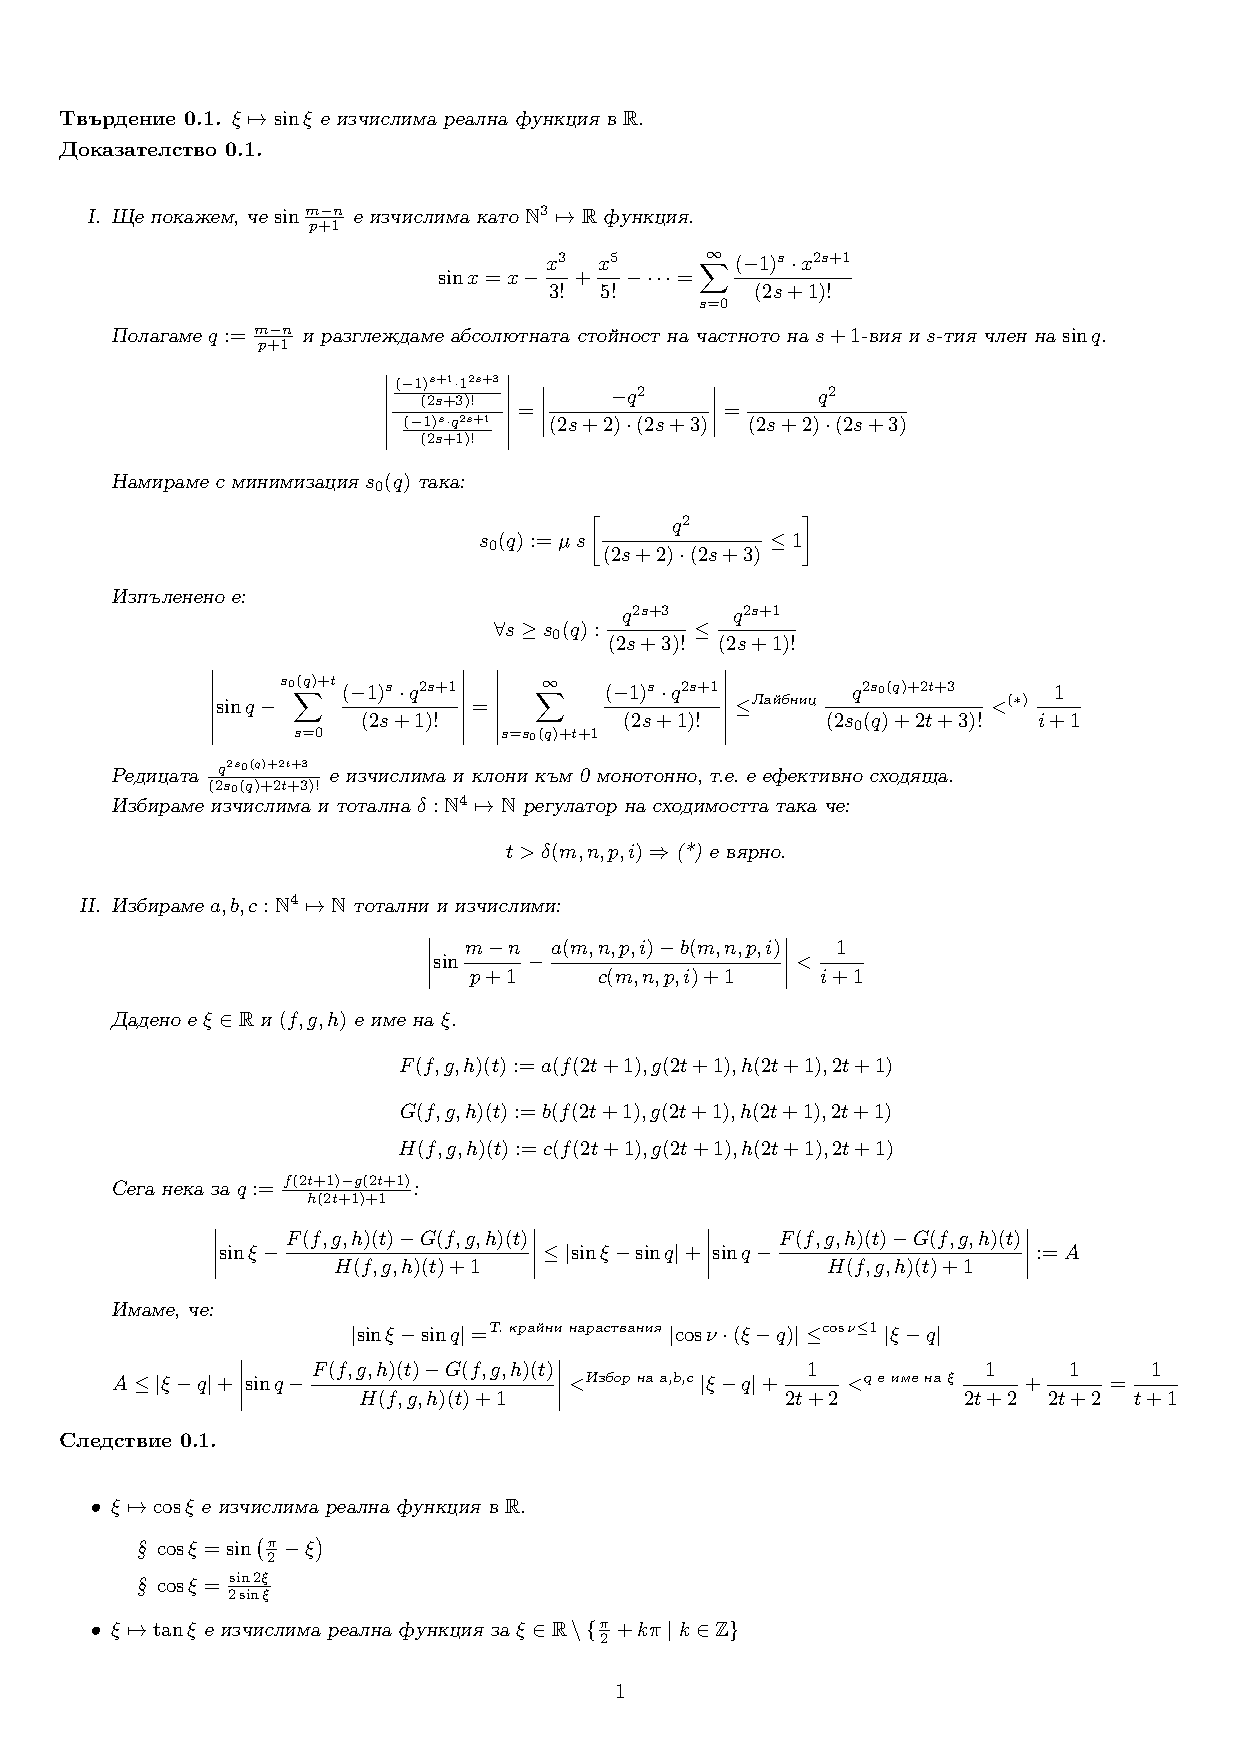
\includepdf{notes/lectures/2024-05-22-Stefanov-computability-of-trig-functions.pdf}